\documentclass[a4paper,11pt]{article}
\usepackage{amsthm,amsmath,amssymb}
\usepackage[citecolor=blue]{hyperref}
\usepackage{color}
\usepackage[table]{xcolor}
\usepackage{tikz}
\usepackage[T1]{fontenc}

\begin{document}

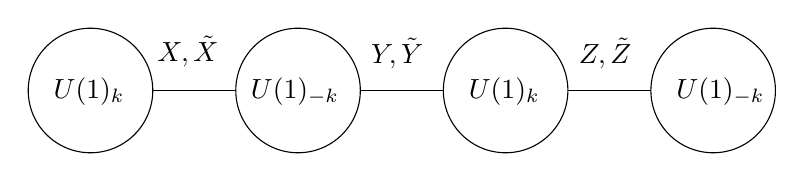
\begin{tikzpicture}[x=0.75pt,y=0.75pt,yscale=-1,xscale=1]

\draw   (10,40) .. controls (10,23.43) and (23.43,10) .. (40,10) .. controls (56.57,10) and (70,23.43) .. (70,40) .. controls (70,56.57) and (56.57,70) .. (40,70) .. controls (23.43,70) and (10,56.57) .. (10,40) -- cycle ;
\draw   (110,40) .. controls (110,23.43) and (123.43,10) .. (140,10) .. controls (156.57,10) and (170,23.43) .. (170,40) .. controls (170,56.57) and (156.57,70) .. (140,70) .. controls (123.43,70) and (110,56.57) .. (110,40) -- cycle ;
\draw   (210,40) .. controls (210,23.43) and (223.43,10) .. (240,10) .. controls (256.57,10) and (270,23.43) .. (270,40) .. controls (270,56.57) and (256.57,70) .. (240,70) .. controls (223.43,70) and (210,56.57) .. (210,40) -- cycle ;
\draw    (70,40) -- (110,40) ;
\draw    (170,40) -- (210,40) ;
\draw   (310,40) .. controls (310,23.43) and (323.43,10) .. (340,10) .. controls (356.57,10) and (370,23.43) .. (370,40) .. controls (370,56.57) and (356.57,70) .. (340,70) .. controls (323.43,70) and (310,56.57) .. (310,40) -- cycle ;
\draw    (270,40) -- (310,40) ;

% Text Node
\draw (21,32.4) node [anchor=north west][inner sep=0.75pt]    {$U( 1)_{k}$};
% Text Node
\draw (221,32.4) node [anchor=north west][inner sep=0.75pt]    {$U( 1)_{k}$};
% Text Node
\draw (116,32.4) node [anchor=north west][inner sep=0.75pt]    {$U( 1)_{-k}$};
% Text Node
\draw (71,12.4) node [anchor=north west][inner sep=0.75pt]    {$X,\tilde{X}$};
% Text Node
\draw (174,13.4) node [anchor=north west][inner sep=0.75pt]    {$Y,\tilde{Y}$};
% Text Node
\draw (321,32.4) node [anchor=north west][inner sep=0.75pt]    {$U( 1)_{-k}$};
% Text Node
\draw (274,13.4) node [anchor=north west][inner sep=0.75pt]    {$Z,\tilde{Z}$};


\end{tikzpicture}

\end{document}